%% LyX 2.3.5.2 created this file.  For more info, see http://www.lyx.org/.
%% Do not edit unless you really know what you are doing.
\documentclass[oneside,UTF8]{ctexbook}
\usepackage[T1]{fontenc}
\setcounter{secnumdepth}{3}
\setcounter{tocdepth}{3}
\usepackage{amsbsy}
\usepackage{amstext}
\usepackage{graphicx}

\makeatletter

%%%%%%%%%%%%%%%%%%%%%%%%%%%%%% LyX specific LaTeX commands.
\newcommand{\noun}[1]{\textsc{#1}}

%%%%%%%%%%%%%%%%%%%%%%%%%%%%%% User specified LaTeX commands.
% 如果没有这一句命令,XeTeX会出错,原因参见
% http://bbs.ctex.org/viewthread.php?tid=60547
% \DeclareRobustCommand\nobreakspace{\leavevmode\nobreak\ }
%%%%%%%%%%%%%%%%%+++++++++++
\usepackage{eso-pic} 
\usepackage{xcolor}
% Required for specifying colors by name 
\definecolor{ocre}{RGB}{243,102,25} 
\usepackage{enumerate} 

\usepackage{amsfonts} 
\usepackage{hep} 
\usepackage{bm} 
\usepackage{graphicx,graphics,color} 
\usepackage{simplewick} 
\usepackage{latexsym} 
\usepackage{amssymb} 
\usepackage{makeidx} 
\usepackage{amsmath} 
\usepackage{multirow} 
\usepackage{slashed} 
%%\usepackage[colorlinks,linkcolor=blue]{hyperref} 
%% \usepackage{axodraw2} 
%%++++++++++++++++++++ 
\DeclareMathOperator{\tr}{Tr} 
\DeclareMathOperator{\re}{Re} 
\DeclareMathOperator{\im}{Im} 
\newcommand*{\dif}{\mathop{}\!\mathrm{d}}

\makeatother

\begin{document}
\title{chpt primer}
\author{Thomas Young}
\maketitle

\chapter{量子色动力学和手征对称性}

\section{SU(3)群的remarks}

SU(3)群在强相互作用中扮演着重要的角色,因为:
\begin{enumerate}
\item 它是量子色动力学(QCD)的规范群
\item 在hadron spectrum中,它基本是一个global的对称性。观察到的(低质量)强子基本上可以填充到SU(3)群的不可约表示中,维数符合,作为简并的多重态。
\item 对于$uds$质量为零的极限,$\text{SU(3)}_{L}\times\text{SU(3)}_{R}$是 QCD 的手征对称性。
\end{enumerate}
因此,先稍微回忆一下,SU(3)群和它的李代数 su(3) 的一些基本性质。

SU(3) 群是所有幺模幺正矩阵群的集合(unitary,unimodular,$3\times3$矩阵)i.e. $U^{\dagger}U=1$,and
$\det(U)=1$。用数学术语说,SU(3)群是 八–参数,简单连接,紧致的\noun{Lie}群。Lie 群的意思群元乘法可以表示成八个解析函数
$U(\Phi_{3})=U(\Phi_{1})U(\Phi_{2})$,其中$\Phi_{3}=\Phi_{3}\left(\Phi_{1},\Phi_{2}\right)$。

是它是 simply-connected,每个群元可以通过参数空间中一条连续的路径连接到恒元,紧致性表示它的参数被限制在有限空间内。对于一个紧致李群,任何一个有限维表示都等价于一个幺正表示,并且可以被分解成不可约表示的直和(Clebsch-Gordan
系数)

SU(3)群的元素可以表示成指数形式
\begin{equation}
U\left(\Theta\right)=\exp\left(-i\sum_{a=1}^{8}\Theta_{a}\frac{\lambda_{a}}{2}\right)=\exp\left(-i\Theta_{a}\frac{\lambda_{a}}{2}\right)\label{eq:1.1}
\end{equation}
其中$\Theta_{a}$是实参数,八个线性独立的矩阵$\lambda_{a}$被称作Gell-Mann 矩阵,满足
\begin{equation}
\frac{\lambda_{a}}{2}=i\frac{\partial U}{\partial\Theta_{a}}\left(0,\cdots,0\right)\label{eq:1.2}
\end{equation}
\begin{equation}
\lambda_{a}=\lambda_{a}^{\dagger}\label{eq:1.3}
\end{equation}
\begin{equation}
\tr\left(\lambda_{a}\lambda_{b}\right)=2\delta_{ab}\label{eq:1.4}
\end{equation}
\begin{equation}
\tr\left(\lambda_{a}\right)=0\label{eq:1.5}
\end{equation}
公式\ref{eq:1.3}负责$U^{\dagger}=U^{-1}$。另一方面,由$\det\left[\exp(C)\right]=\exp\left[\tr(C)\right]$,公式\ref{eq:1.5}导致$\det(U)=1$。如果$U$矩阵是幺正的,那么其实相当于要求指数上的因子是反厄米(skew-hermitian
)的,就是$A=-A^{\dagger}$。这个负号由虚数单位$i$来负责,所以盖尔曼矩阵是厄米的。

Gell-Mann 矩阵的一个显式表示为:
\[
\begin{array}{ccc}
\lambda_{1}=\left(\begin{array}{ccc}
0 & 1 & 0\\
1 & 0 & 0\\
0 & 0 & 0
\end{array}\right) & \lambda_{2}=\left(\begin{array}{ccc}
0 & -i & 0\\
i & 0 & 0\\
0 & 0 & 0
\end{array}\right) & \lambda_{3}=\left(\begin{array}{ccc}
1 & 0 & 0\\
0 & -1 & 0\\
0 & 0 & 0
\end{array}\right)\\
\lambda_{4}=\left(\begin{array}{ccc}
0 & 0 & 1\\
0 & 0 & 0\\
1 & 0 & 0
\end{array}\right) & \lambda_{5}=\left(\begin{array}{ccc}
0 & 0 & -i\\
0 & 0 & 0\\
i & 0 & 0
\end{array}\right) & \lambda_{6}=\left(\begin{array}{ccc}
0 & 0 & 0\\
0 & 0 & 1\\
0 & 1 & 0
\end{array}\right)\\
\lambda_{7}=\left(\begin{array}{ccc}
0 & 0 & 0\\
0 & 0 & -i\\
0 & i & 0
\end{array}\right) & \lambda_{8}=\sqrt{\frac{1}{3}}\left(\begin{array}{ccc}
1 & 0 & 0\\
0 & 1 & 0\\
0 & 0 & -2
\end{array}\right)
\end{array}
\]
集合$\left\{ i\lambda_{a}\vert a=1,\cdots,8\right\} $组成了su(3) 李代数的基,即,所有的复的,无迹的,反厄米的,$3\times3$矩阵。李乘积定义为两个矩阵的对易子。这样的定义自然满足李的反对易性。
\[
\left[A,B\right]=-\left[B,A\right]
\]
还有jacobi 恒等式
\[
\left[A,\left[B,C\right]\right]+\left[B,\left[C,A\right]\right]+\left[C,\left[A,B\right]\right]=0
\]
与式\ref{eq:1.1}和\ref{eq:1.2}兼容。su(3)的元素可以理解为SU(3)恒元附近的切矢量。

李群的结构被encoded在盖尔曼矩阵的对易关系中
\[
\left[\frac{\lambda_{a}}{2},\frac{\lambda_{b}}{2}\right]=if_{abc}\frac{\lambda_{c}}{2}
\]
全反对称实的结构常数$f_{abc}$可以从式\ref{eq:1.4}获取
\[
f_{abc}=\frac{1}{4i}\tr\left(\left[\lambda_{a},\lambda_{b}\right]\lambda_{c}\right)
\]
粗略地说,结构常数表征了SU(3)群不对易的程度。不为零的分量在表格\ref{fig:=008868=00683C1.1}中给出
\begin{figure}
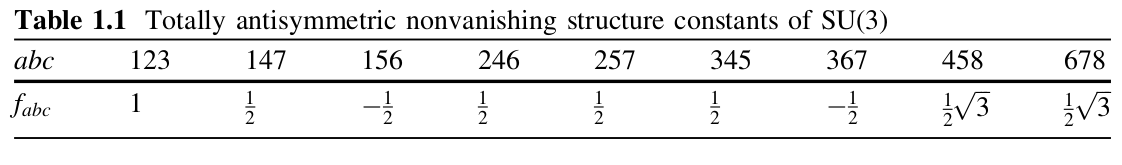
\includegraphics[scale=0.46]{pasted1}

\caption{表格1.1\label{fig:=008868=00683C1.1}}

\end{figure}

盖尔曼矩阵的反对易关系是
\[
\left\{ \lambda_{a},\lambda_{b}\right\} =\frac{4}{3}\delta_{ab}\boldsymbol{1}+2d_{abc}\lambda_{c}
\]
其中全对陈张量$d_{abc}$由下式给出
\[
d_{abc}=\frac{1}{4}\tr\left(\left\{ \lambda_{a},\lambda_{b}\right\} \lambda_{c}\right)
\]
在表格\ref{fig:=008868=00683C1.2}中给出
\begin{figure}
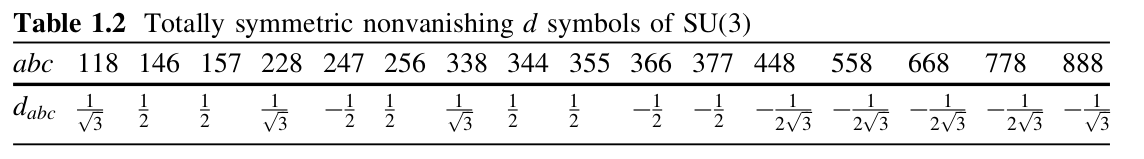
\includegraphics[scale=0.46]{pasted2}

\caption{表格1.2\label{fig:=008868=00683C1.2}}

\end{figure}

很明显,盖尔曼矩阵的反对易并不一定是盖尔曼矩阵。因为反厄密矩阵的平方不再反厄米。

end of file

end of file
\begin{thebibliography}{1}
\bibitem{ref61}ref61
\end{thebibliography}

\end{document}
